\section{Sensitivity Analysis} \label{appendix:sensitivity}

\noindent This appendix evaluates how the estimates in the main paper vary as we alter certain
sample selections from all of our data sources and other parameters. We analyze sensitivity due to (i) assumptions on the values of the discount rate; (ii) assumptions on the deadweight loss to society coming from taxes raised to fund public programs; and (iii) the magnitude of the components contributing to the benefit/cost ratio and internal rate of return. \\


\subsection{Varying the Discount Rate}

%In this section we explore how the internal rate of return and benefit/cost ratio
%change when we adjust various components of the cash flow, as well as various parameters
%we assume. Not only does this provide us with an idea of how stable our estimates 
%are, but also which components or assumptions are responsible for any instabilities
%we find in our estimates.

\noindent Below we examine how the benefit/cost ratio is impacted by our choice of the discount rate. \\

\noindent Figure \ref{fig:bcr_discount} displays how the benefit/cost ratio changes as we adjust
the rate at which we discount the cash flows. We find that for males, the benefits of 
the programs exceed the costs for discount rates as high as 12\%. We also
find that the benefit/cost ratios for discount rates of 2--12\% remain within the 
80\% confidence interval of our actual point estimate. The case is different for females,
for whom the ratio falls below 1 at a discount rate of 6\%. The benefit/cost ratio for 
females remain within the 80\% confidence interval of our estimate for discount rates
of 2--15\%. Although the alternate estimates generally remain within the 80\%
confidence intervals for both males and females, the slope of the curves in Figure
\ref{fig:bcr_discount} indicate that our estimates are sensitive to our choice of
the discount rate, especially for males. 

\begin{figure}[H]
\caption{Benefit/cost Ratio vs. Discount Rate} \label{fig:bcr_discount}
	\begin{subfigure}[h]{0.8\textwidth}
	\centering
	\caption{Females} \label{fig:bcr_discount_f1}
	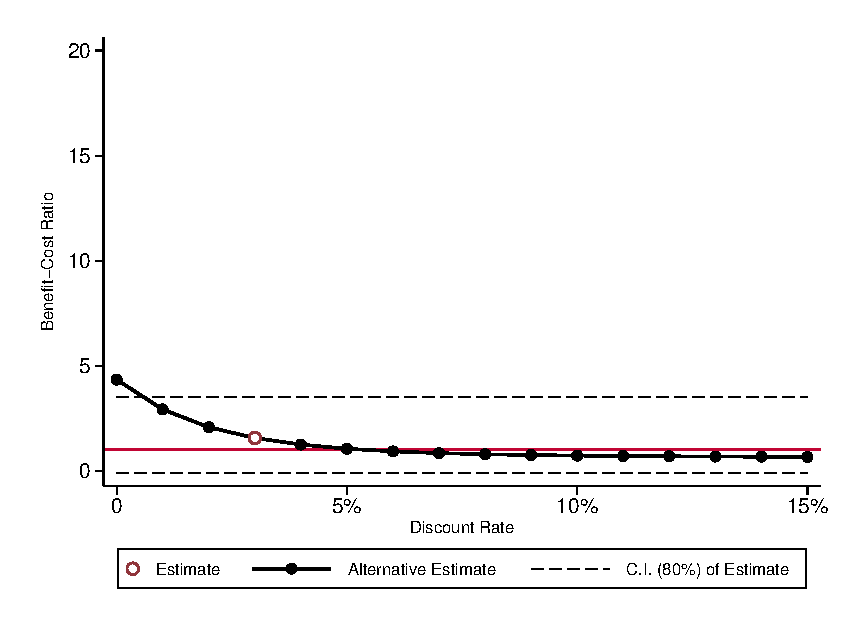
\includegraphics[width=\textwidth]{AppOutput/Sensitivity/bcr_discount_f1.eps}
	\end{subfigure}
	
	\begin{subfigure}[h]{0.8\textwidth}
	\centering
	\caption{Males} \label{fig:bcr_discount_m}
	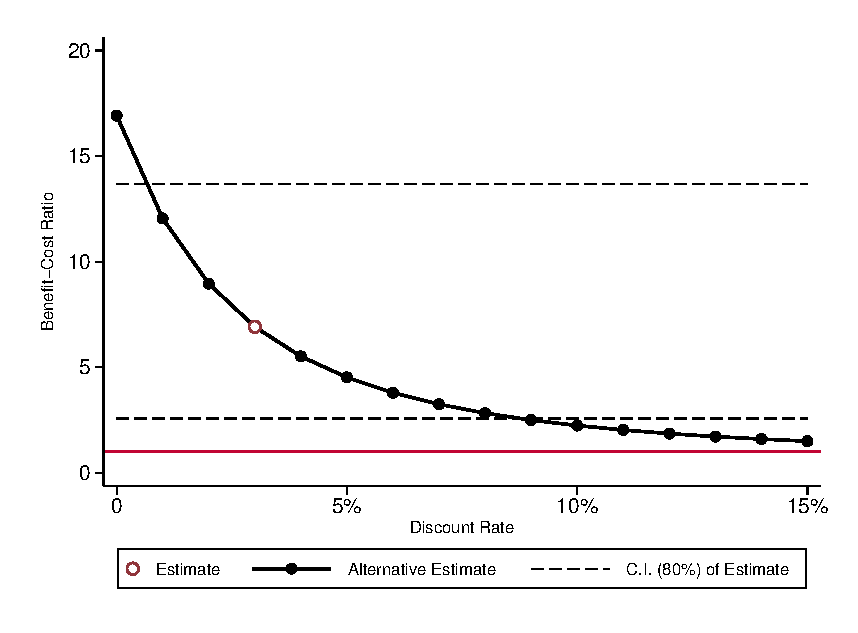
\includegraphics[width=\textwidth]{AppOutput/Sensitivity/bcr_discount_m1.eps}
	\end{subfigure}
	\floatfoot{
	\noindent Note: These graphs display how the benefit/cost ratios change
	for females and males as we vary the rate at which we discount to obtain the 
	present value. 
	The red line indicates a benefit/cost ratio of 1. 
	The hollow circle represents our actual estimates, whereas the
	solid dots represent the alternative estimates we obtain by varying the discount rate. 
	The estimates presented in the paper assume that the marginal 
	cost of welfare is \$0.50 for every dollar of tax revenue. 
	The estimates are means of the empirical bootstrap 
	distribution. The 80\% confidence intervals are obtained by taking the 10\textsuperscript{th}
	and 90\textsuperscript{th} quantiles of the bootstrap distribution.
	}
\end{figure}


\subsection{Varying Deadweight Loss}

\noindent Below we examine how our estimates of the internal rate of return (IRR) and benefit/cost
ratios move with respect to changes in the marginal cost of welfare. \\

\noindent Figure \ref{fig:irr_dwl} shows how the IRR changes as we adjust
the marginal cost of welfare. For both males and females, we find the IRRs
to be most sensitive at the lower marginal costs. The IRRs for both sexes
steadily decline as we increase the marginal cost of welfare to \$3 for every dollar
of tax revenue. This is likely due
to the fact that both females and males in treatment live longer, and are expected to 
receive more Medicare and Medicaid benefits in their later life. 
Also, we treat the costs of implementing ABC/CARE as a public cost. 
Thus, the steady increase in deadweight loss results in a 
steady decline in the IRR. Nonetheless, we see that the IRRs 
remain within the 80\% confidence interval of our original estimate 
for both females and males and are not particularly sensitive to changes within the 
neighborhood of our assumed marginal cost of welfare (note each point on the $x$-axis
represents a \$0.25 increment in the cost of welfare per dollar of tax revenue). 


\begin{figure}[H]
\caption{Internal Rate of Return vs. Deadweight Loss} \label{fig:irr_dwl}
	\begin{subfigure}[h]{0.8\textwidth}
	\centering
	\caption{Females} \label{fig:irr_dwl_f}
	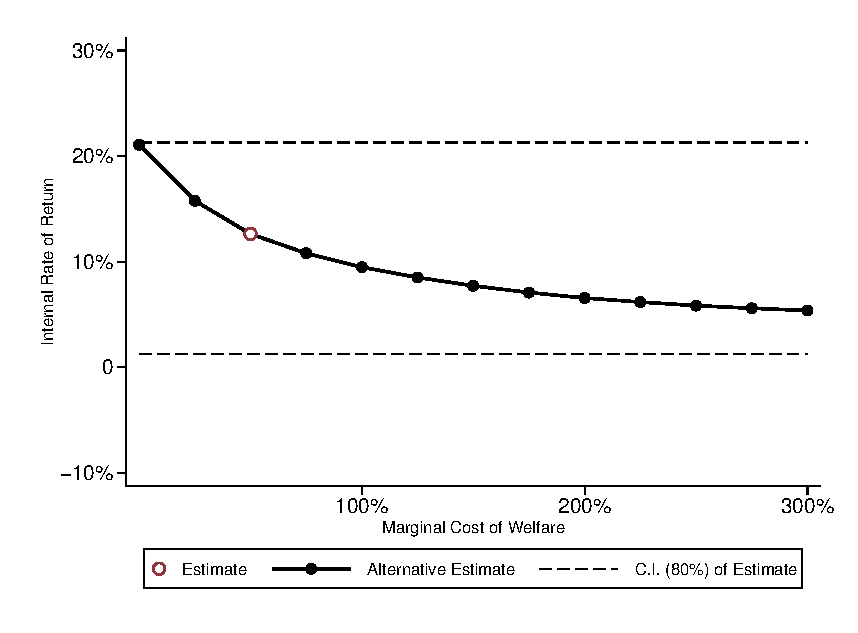
\includegraphics[width=\textwidth]{AppOutput/Sensitivity/irr_dwl_f1.eps}
	\end{subfigure}
	
	\begin{subfigure}[h]{0.8\textwidth}
	\centering
	\caption{Males} \label{fig:irr_dwl_m}
	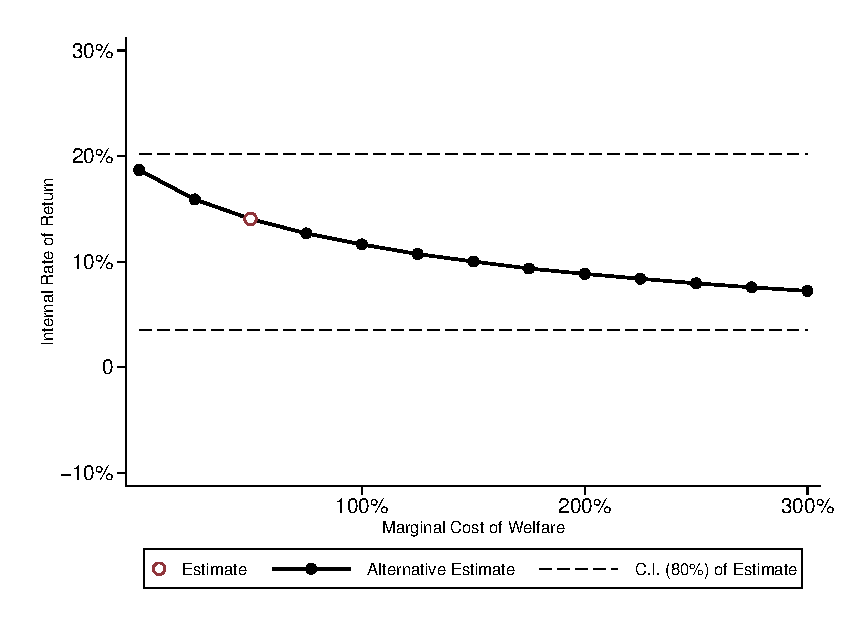
\includegraphics[width=\textwidth]{AppOutput/Sensitivity/irr_dwl_m1.eps}
	\end{subfigure}
	\floatfoot{
	\noindent Note: These graphs display how the internal rate of return changes
	for females and males as we vary the marginal cost of welfare.
	The hollow circle represents our actual estimates, whereas the
	solid dots represent the alternative estimates we obtain by varying the marginal
	cost of welfare. The estimates 
	presented in the paper assume that the marginal cost of welfare is \$0.50 for 
	every dollar of tax revenue. The estimates are means of the empirical bootstrap 
	distribution. The 80\% confidence intervals are obtained by taking the 10\textsuperscript{th}
	and 90\textsuperscript{th} quantiles of the bootstrap distribution.
	}
\end{figure}

\noindent Figure \ref{fig:bcr_dwl} illustrates how the benefit/cost ratio changes as we vary
the marginal cost of welfare. For females we see that the costs continue to exceed the benefits (both are discounted at a rate of 4\%) even when the marginal cost of welfare is
assumed to equal \$1 for every dollar of tax revenue. For males, the benefits
exceed the costs even as we increase the deadweight loss to \$3 for every dollar of tax
revenue. The resilience of the benefit/cost ratio of males is attributed to the 
large impacts ABC/CARE had on criminal activity, which bears a large cost to society. As we
increase the marginal cost of welfare, we are in fact increasing the stream of benefits
associated with the reduction in criminal costs of males. At the same time, however,
we are also increasing the later-life public medical costs associated with Medicare
and Medicaid, as well as the program costs. 

\begin{figure}[H]
\caption{Benefit/cost Ratio vs. Deadweight Loss} \label{fig:bcr_dwl}
	\begin{subfigure}[h]{0.8\textwidth}
	\centering
	\caption{Females} \label{fig:bcr_dwl_f}
	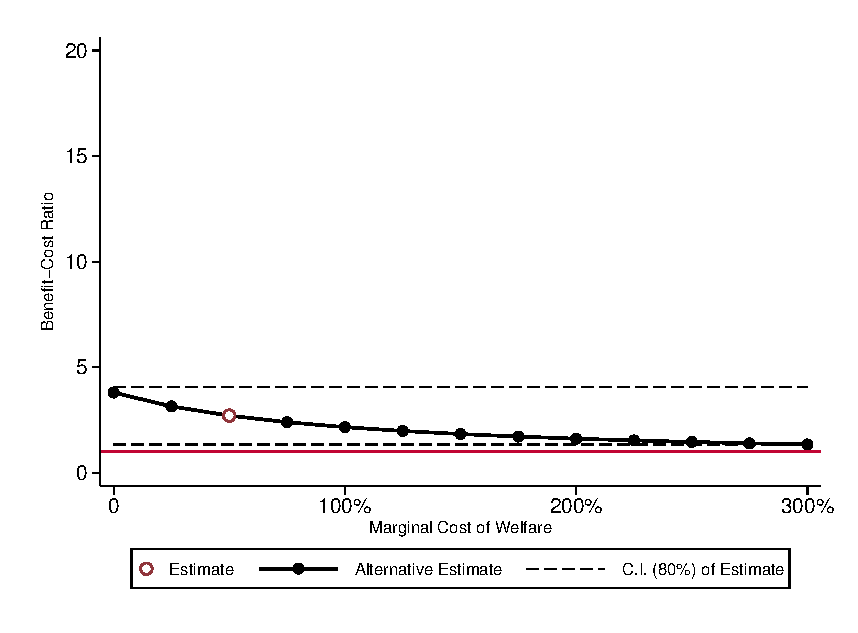
\includegraphics[width=\textwidth]{AppOutput/Sensitivity/bcr_dwl_f1.eps}
	\end{subfigure}
	
	\begin{subfigure}[h]{0.8\textwidth}
	\centering
	\caption{Males} \label{fig:bcr_dwl_m}
	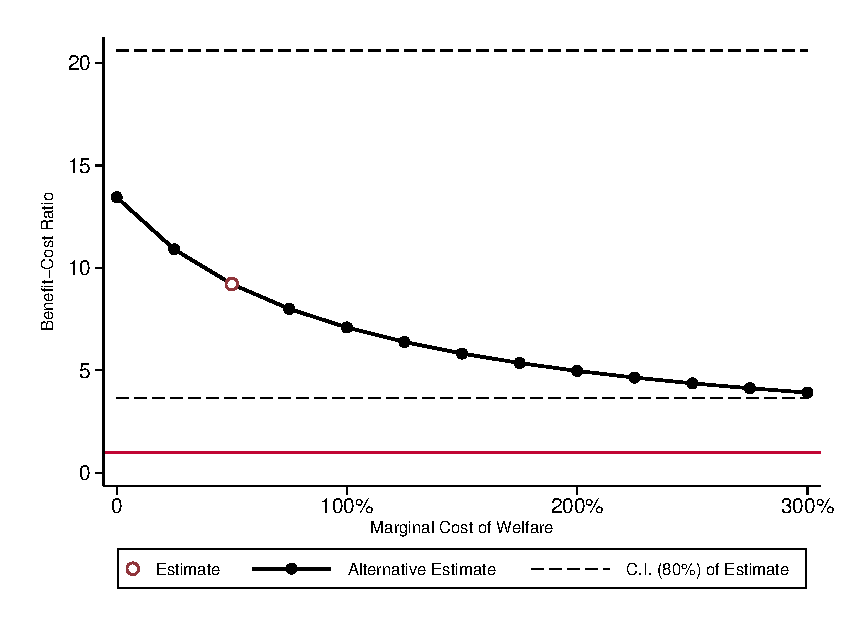
\includegraphics[width=\textwidth]{AppOutput/Sensitivity/bcr_dwl_m1.eps}
	\end{subfigure}
	\floatfoot{
	\noindent Note: These graphs display how the benefit/cost ratio changes
	for females and males as we vary the marginal cost of welfare.  
	The red line indicates a benefit/cost ratio of 1. 
	The hollow circle represents our actual estimates, whereas the
	solid dots represent the alternative estimates we obtain by varying the marginal
	cost of welfare. The estimates 
	presented in the paper assume that the marginal cost of welfare is \$0.50 for 
	every dollar of tax revenue. The estimates are means of the empirical bootstrap 
	distribution. The 80\% confidence intervals are obtained by taking the 10\textsuperscript{th}
	and 90\textsuperscript{th} quantiles of the bootstrap distribution.
	}
\end{figure}

\subsection{Varying Component Magnitudes}
\label{app:sa_factors}

\noindent Below we explore how the internal rate of return (IRR) and benefit/cost ratio change as
we increase and decrease the value of each component of the benefit and cost streams. This entails
multiplying each component by factors ranging from 0 to 3. A factor of 0 is equivalent
to removing the component entirely from our analysis. In the particular
case of QALYs, the multiplicative factors correspond to different valuations of a year of perfect
health, e.g., a QALY equal to 1. For instance, as our current estimates assume a QALY of 1 to be worth
\$150,000, a factor of 0.5 corresponds to a year of perfect health being
worth \$75,000, and a factor of 3 corresponds to a year of perfect health
being worth \$450,000 (all values are in 2014 USD). \\

\noindent Figure \ref{fig:irrf_factor_f} displays how the IRR for females
changes as we multiply each component by a factor between 0 and 3. We find that the IRR
is stable across different levels of public-transfer income, QALYs, health costs, and criminal 
costs. Parental income has the biggest effect on the IRR, 
and is one of the only components for which the alternative IRR falls outside of the 80\% confidence 
interval of the original estimate. This occurs when we double the parental income component in the
flow of benefits. By tripling the component, we obtain an IRR exceeding 100\%, which we
do not display in the chart above. This sensitivity is due to both the magnitude of the
treatment effect on parental income, as well as how the treatment effect took place
earlier in the ABC/CARE subjects' lives. The sensitivity of the IRR to the program costs
is also a result of the timing of the costs in the subjects lives. As females in the treatment groups attained higher levels of education
than females in the control groups, we observe that the IRR decreases as we multiply the
expenditure on education by increasingly large factors. On the other hand, this translates
to additional labor income for females, which we observe to have a positive effect on the
IRR. However, the IRR appears to be more sensitive to the costs of education relative
to labor income, as schooling costs are borne at earlier stages of each subject's life. 


\begin{figure}[H]
\caption{Internal Rate of Return vs.~Components, Females} \label{fig:irrf_factor_f}
	
	\begin{subfigure}[h]{0.8\textwidth}
	\centering
	\caption{Labor Income} \label{fig:irrf_inc_labor_f1}
	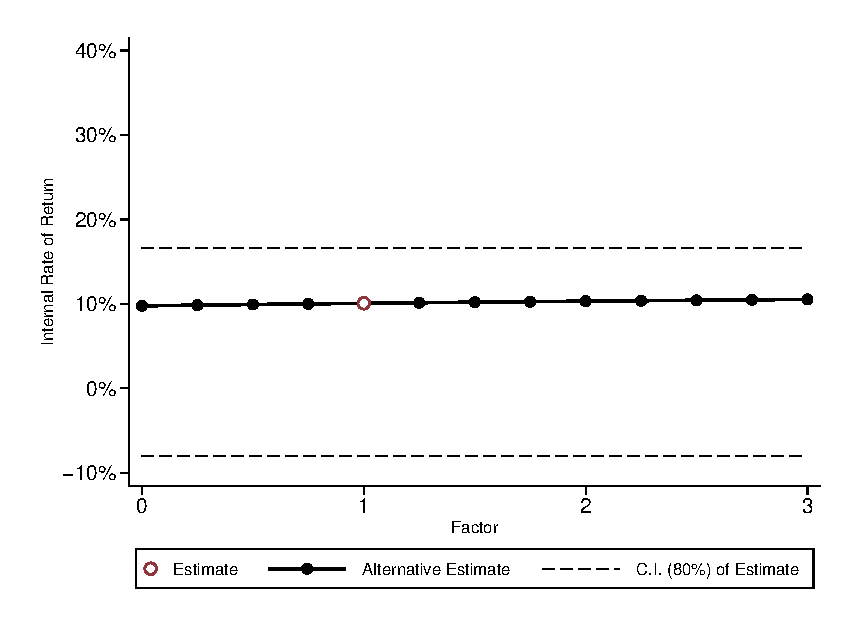
\includegraphics[width=\textwidth]{AppOutput/Sensitivity/irrf_inc_labor_f1.eps}
	\end{subfigure}
	
	\begin{subfigure}[h]{0.8\textwidth}
	\centering
	\caption{Public-Transfer Income} \label{fig:irrf_transfer_f1}
	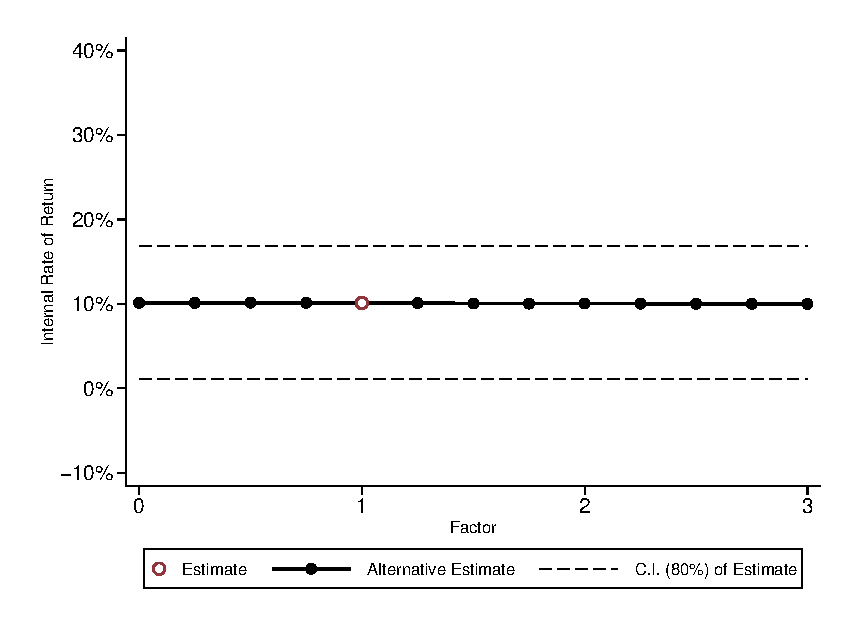
\includegraphics[width=\textwidth]{AppOutput/Sensitivity/irrf_transfer_f1.eps}
	\end{subfigure}
\end{figure}

\begin{figure}[H]
\ContinuedFloat	
	\begin{subfigure}[h]{0.8\textwidth}
	\centering
	\caption{Parental Income} \label{fig:irrf_inc_parent_f1}
	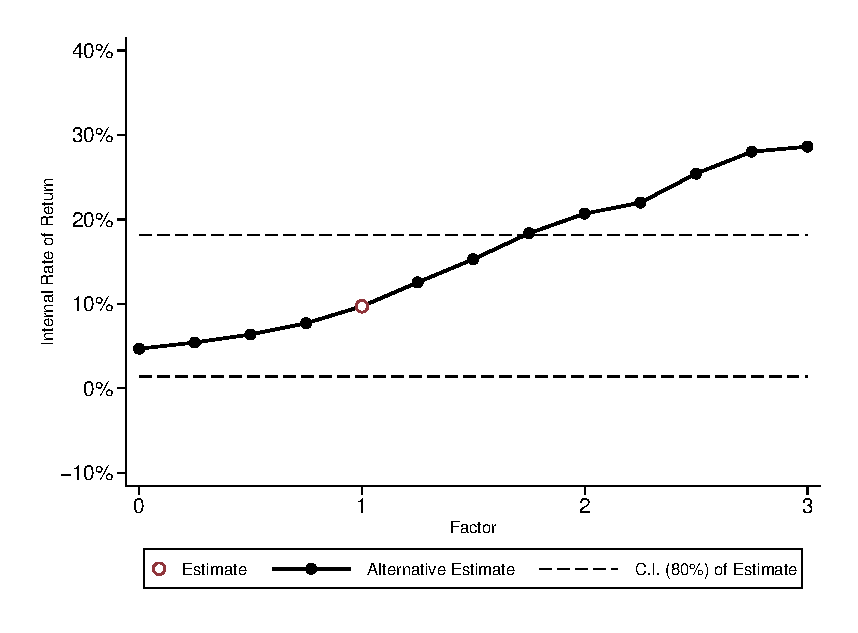
\includegraphics[width=\textwidth]{AppOutput/Sensitivity/irrf_inc_parent_f1.eps}
	\end{subfigure}
	
	\begin{subfigure}[h]{0.8\textwidth}
	\centering
	\caption{Quality-Adjusted Life Years} \label{fig:irrf_qaly_f1}
	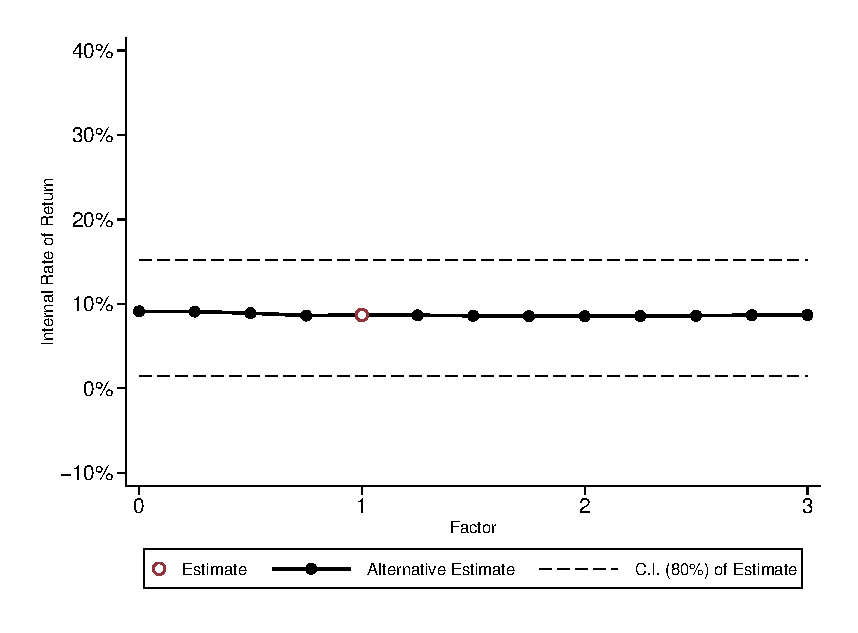
\includegraphics[width=\textwidth]{AppOutput/Sensitivity/irrf_qaly_f1.eps}
	\end{subfigure}
\end{figure}
	
\begin{figure}[H]
\ContinuedFloat	
	\begin{subfigure}[h]{0.8\textwidth}
	\centering
	\caption{Health Costs} \label{fig:irrf_health_f1}
	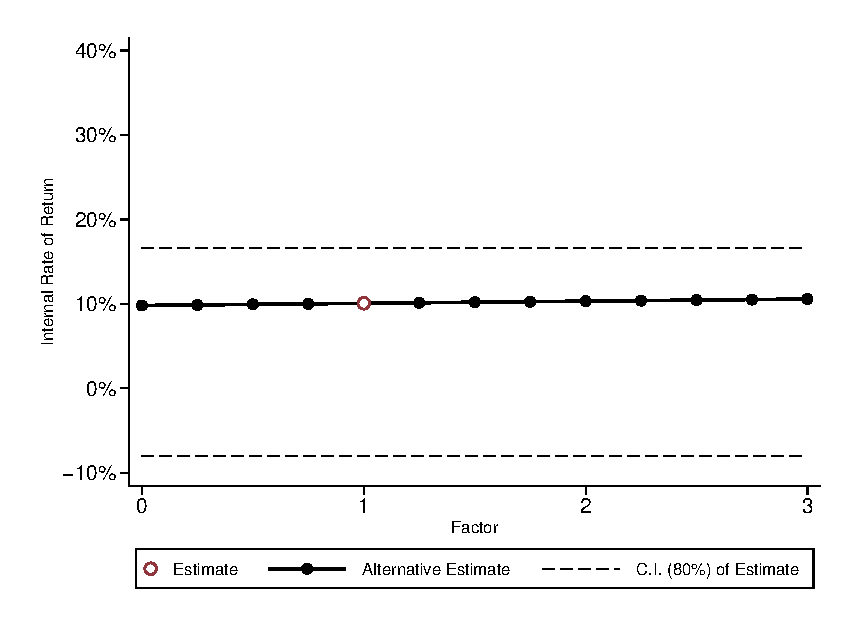
\includegraphics[width=\textwidth]{AppOutput/Sensitivity/irrf_health_f1.eps}
	\end{subfigure}
	
	\begin{subfigure}[h]{0.8\textwidth}
	\centering
	\caption{Education Costs} \label{fig:irrf_edu_f1}
	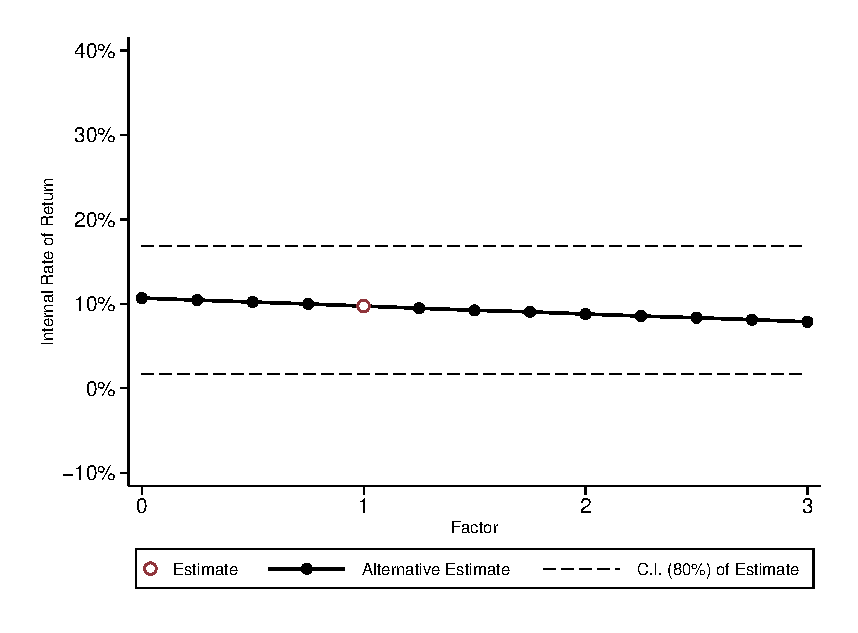
\includegraphics[width=\textwidth]{AppOutput/Sensitivity/irrf_edu_f1.eps}
	\end{subfigure}
\end{figure}

\begin{figure}[H]
\ContinuedFloat	
	\begin{subfigure}[h]{0.8\textwidth}
	\centering
	\caption{Crime Costs} \label{fig:irrf_crime_f1}
	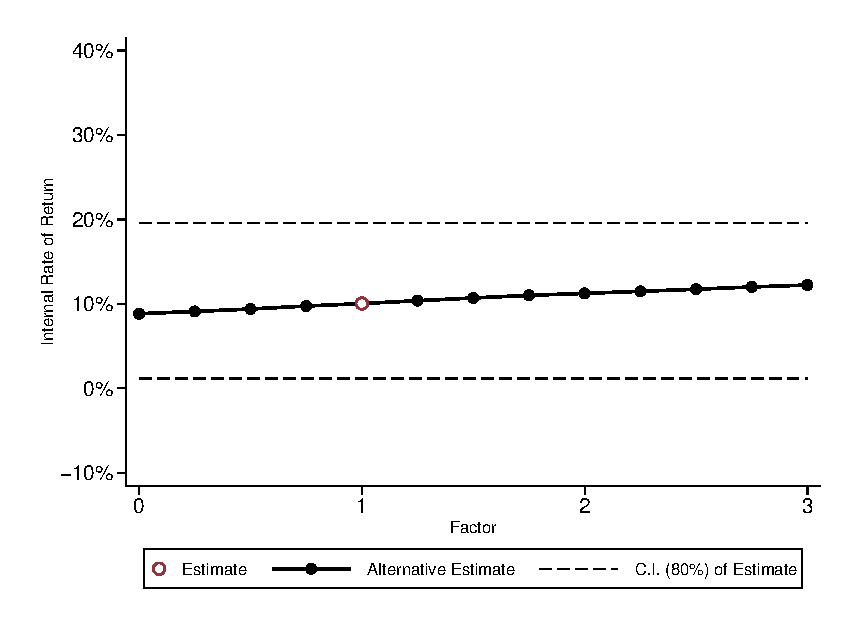
\includegraphics[width=\textwidth]{AppOutput/Sensitivity/irrf_crime_f1.eps}
	\end{subfigure}
	
	\begin{subfigure}[h]{0.8\textwidth}
	\centering
	\caption{Program Costs} \label{fig:irrf_costs_f1}
	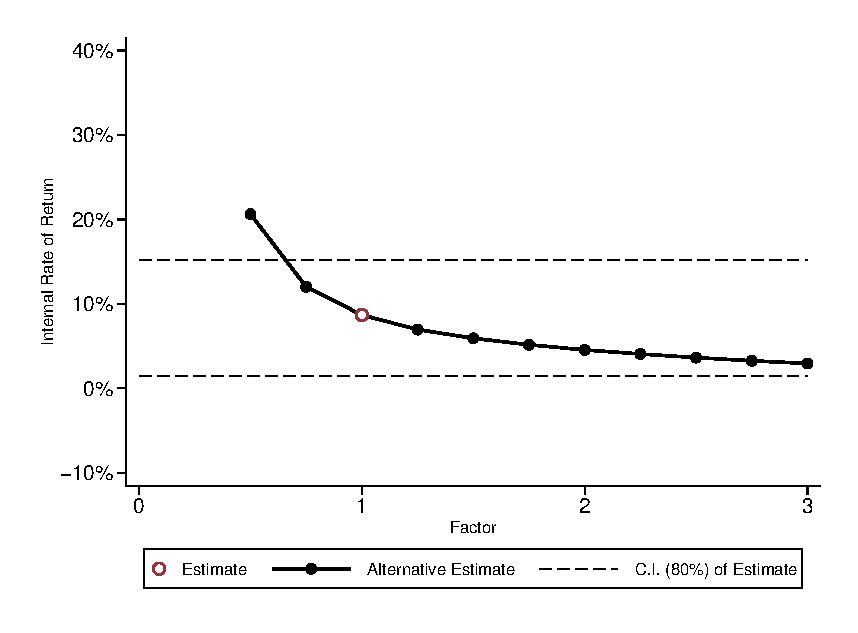
\includegraphics[width=\textwidth]{AppOutput/Sensitivity/irrf_costs_f1.eps}
	\end{subfigure}
\end{figure}
	
\begin{figure}[H]
\ContinuedFloat	
	\begin{subfigure}[h]{0.8\textwidth}
	\centering
	\caption{Control Substitution Costs} \label{fig:irrf_cc_f1}
	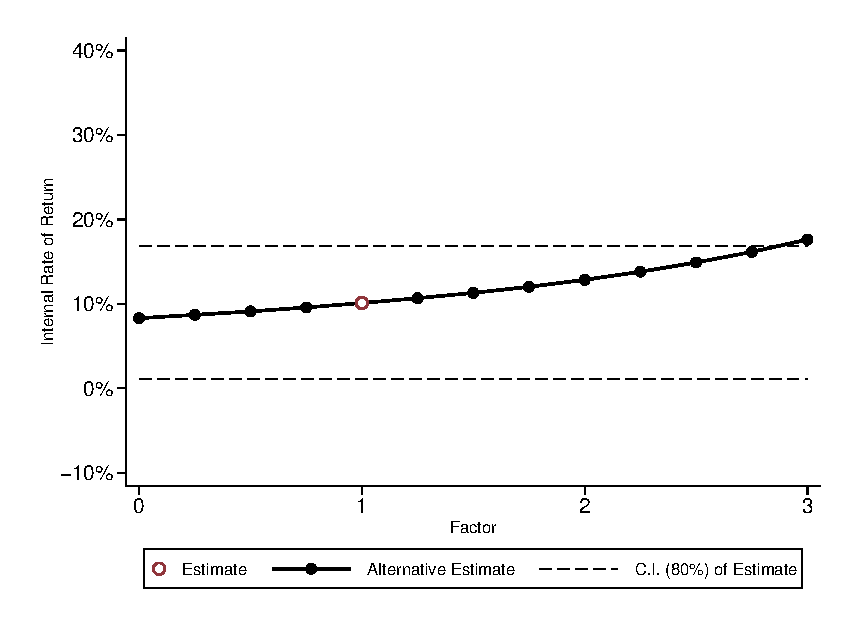
\includegraphics[width=\textwidth]{AppOutput/Sensitivity/irrf_cc_f1.eps}
	\end{subfigure}
	
	\floatfoot{
	\noindent Note: These graphs display how the internal rate of return changes
	for females as we multiply each component by a factor from 0 to 3. 
	The hollow circle represents our actual estimates, whereas the
	solid dots represent the alternative estimates we obtain by varying the 
	magnitude of each component. The estimates 
	presented in the paper are equal to the IRRs presented above when the multiplicative
	factor is equal to 1. The estimates are means of the empirical bootstrap 
	distribution. The 80\% confidence intervals are obtained by taking the 10\textsuperscript{th}
	and 90\textsuperscript{th} quantiles of the bootstrap distribution.
	}
\end{figure}

\noindent Figure \ref{fig:irrf_factor_m} displays how the IRR for males changes as we vary the magnitude
of each component of the benefits and costs. Our findings for males are similar to
those for females: the IRR is insensitive to changes in public-transfer income, QALYs, and health costs. 
As the parental income and the program cost components for the female subsample is 
the same as those of the male subsample, we also observe that the IRR for males 
is sensitive to changes in both of these components. The IRR for males is similarly sensitive to increasing the weight of the cost of control substitution. Compared to females, however, as the weight increases, the internal rate of return increases at a much faster rate. This is a product of the different populations of males and females who were enrolled in alternative preschools.
The IRR for the male subsample is a little less sensitive to changes in labor income
and education costs than for the female subsample, but we still observe in Figure \ref{fig:irrf_factor_m}
that the IRR for males rises as we multiply the benefits stemming from those components 
by increasingly large factors. 
Finally, the IRR steadily 
increases for males as we increase the magnitude of the criminal cost component. 
This is not surprising because the reduction in the costs of crimes is the largest 
benefit of ABC/CARE for males. 


\begin{figure}[H]
\caption{Internal Rate of Return vs.~Components, Males} \label{fig:irrf_factor_m}
	\begin{subfigure}[h]{0.8\textwidth}
	\centering
	\caption{Labor Income} \label{fig:irrf_inc_labor_m1}
	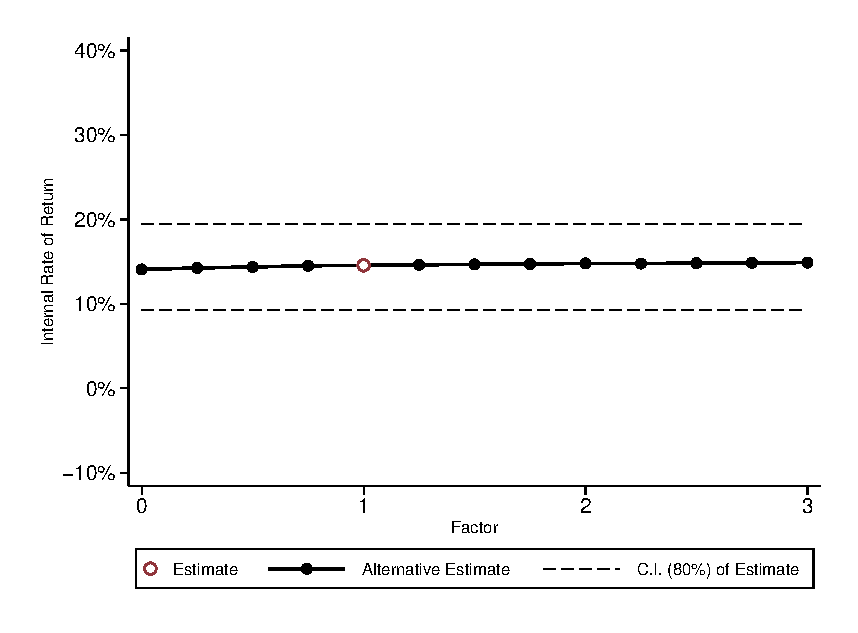
\includegraphics[width=\textwidth]{AppOutput/Sensitivity/irrf_inc_labor_m1.eps}
	\end{subfigure}	
	
	\begin{subfigure}[h]{0.8\textwidth}
	\centering
	\caption{Public-Transfer Income} \label{fig:irrf_transfer_m1}
	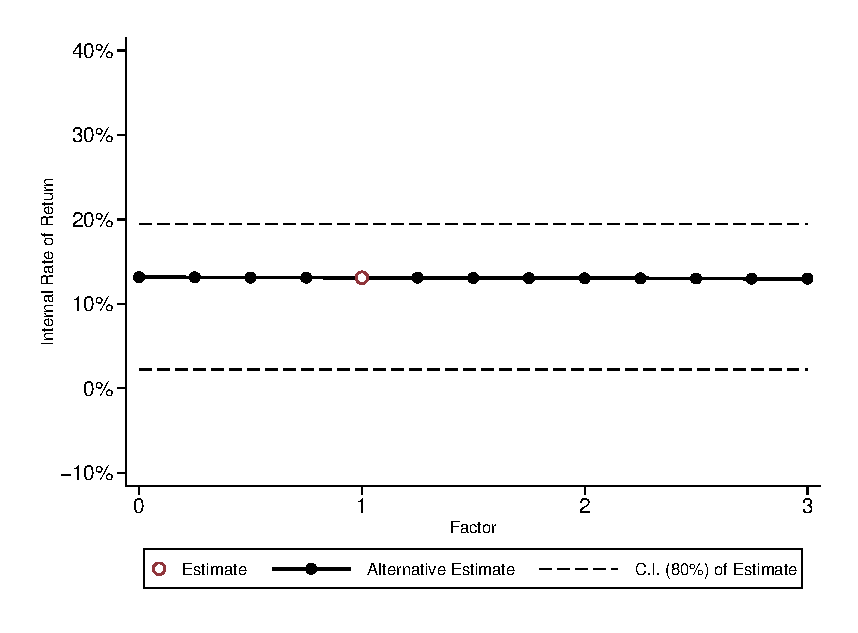
\includegraphics[width=\textwidth]{AppOutput/Sensitivity/irrf_transfer_m1.eps}
	\end{subfigure}
\end{figure}
	
\begin{figure}[H]
\ContinuedFloat		
	\begin{subfigure}[h]{0.8\textwidth}
	\centering
	\caption{Parental Income} \label{fig:irrf_inc_parent_m1}
	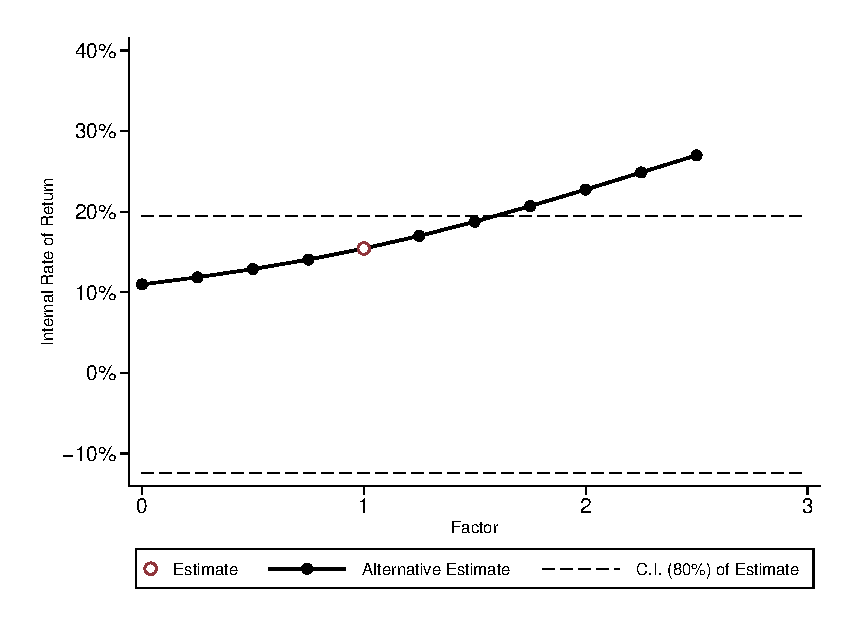
\includegraphics[width=\textwidth]{AppOutput/Sensitivity/irrf_inc_parent_m1.eps}
	\end{subfigure}
	
	\begin{subfigure}[h]{0.8\textwidth}
	\centering
	\caption{Quality-Adjusted Life Years} \label{fig:irrf_qaly_m1}
	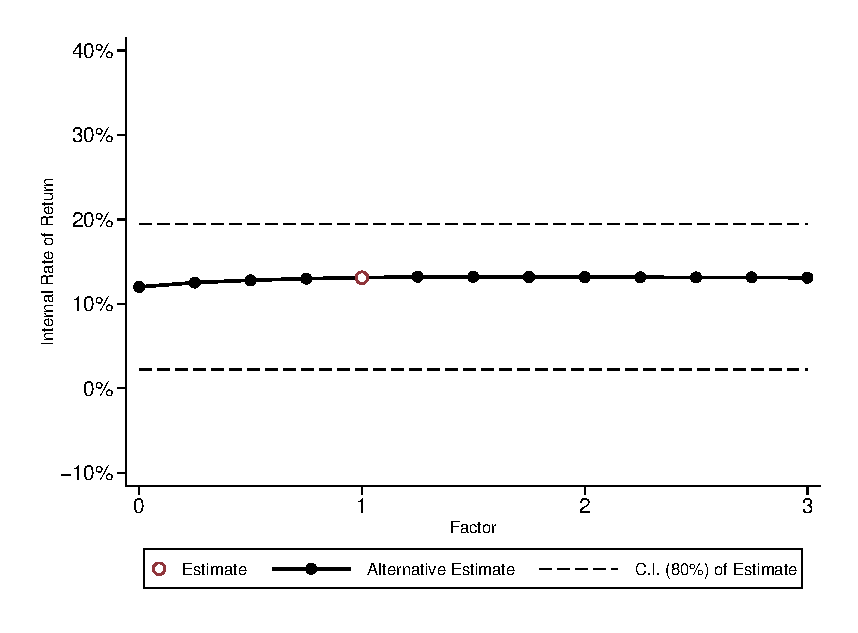
\includegraphics[width=\textwidth]{AppOutput/Sensitivity/irrf_qaly_m1.eps}
	\end{subfigure}
\end{figure}
	
\begin{figure}[H]
\ContinuedFloat		
	\begin{subfigure}[h]{0.8\textwidth}
	\centering
	\caption{Health Costs} \label{fig:irrf_health_m1}
	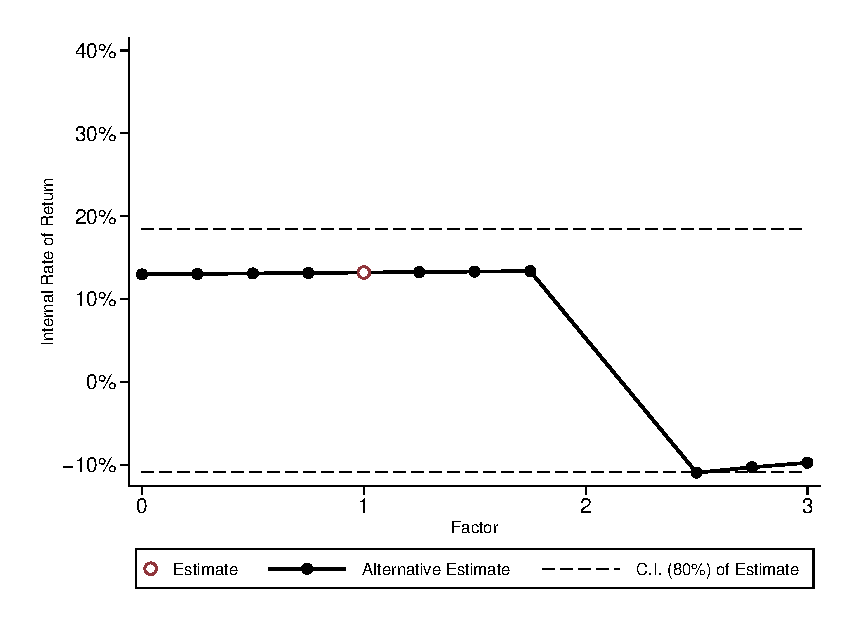
\includegraphics[width=\textwidth]{AppOutput/Sensitivity/irrf_health_m1.eps}
	\end{subfigure}
	
	\begin{subfigure}[h]{0.8\textwidth}
	\centering
	\caption{Education Costs} \label{fig:irrf_edu_m1}
	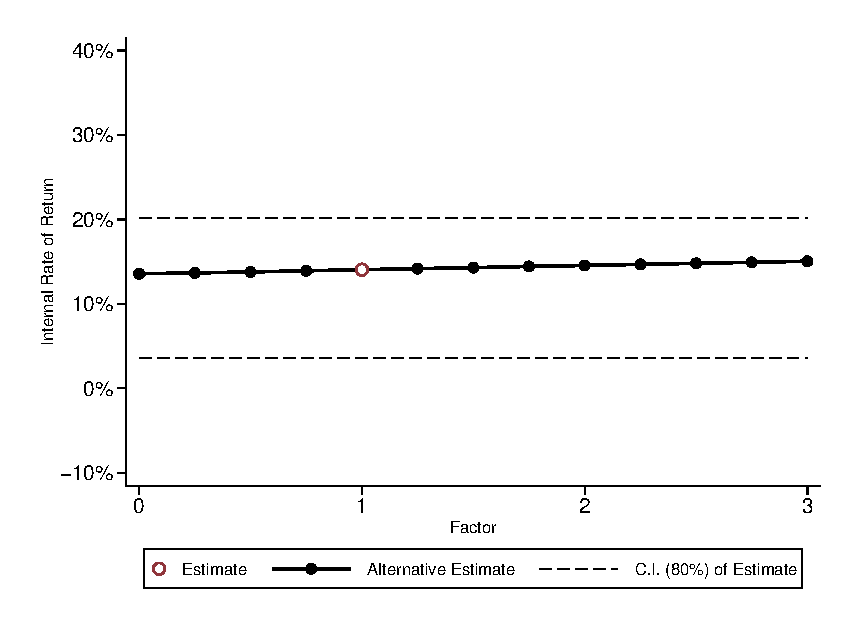
\includegraphics[width=\textwidth]{AppOutput/Sensitivity/irrf_edu_m1.eps}
	\end{subfigure}
\end{figure}
	
\begin{figure}[H]
\ContinuedFloat		
	\begin{subfigure}[h]{0.8\textwidth}
	\centering
	\caption{Crime Costs} \label{fig:irrf_crime_m1}
	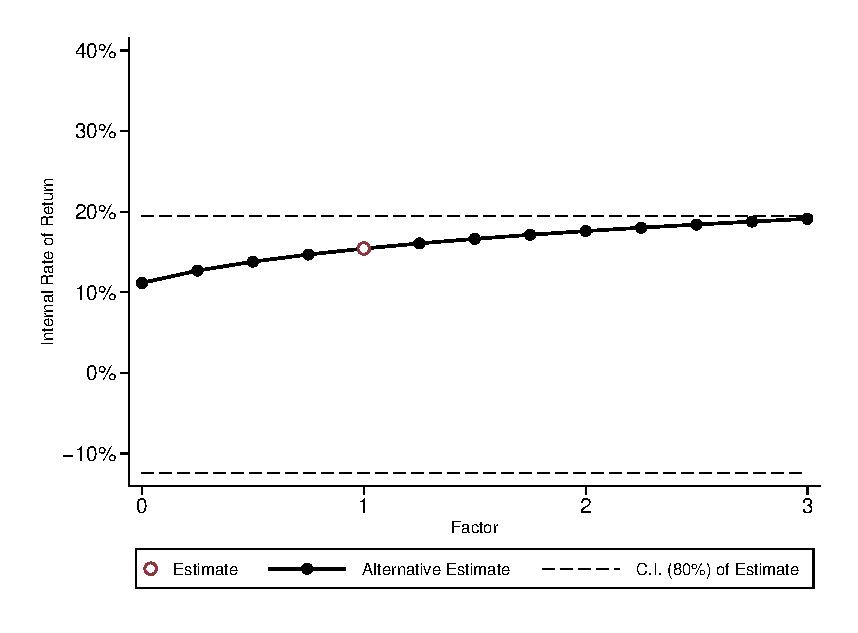
\includegraphics[width=\textwidth]{AppOutput/Sensitivity/irrf_crime_m1.eps}
	\end{subfigure}
	
	\begin{subfigure}[h]{0.8\textwidth}
	\centering
	\caption{Program Costs} \label{fig:irrf_costs_m1}
	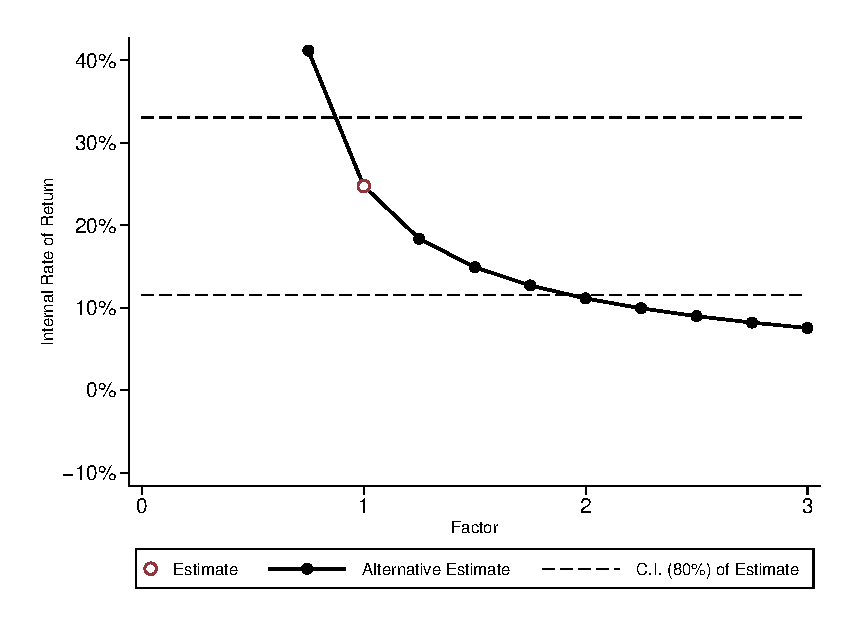
\includegraphics[width=\textwidth]{AppOutput/Sensitivity/irrf_costs_m1.eps}
	\end{subfigure}
\end{figure}
	
\begin{figure}[H]
\ContinuedFloat		
	\begin{subfigure}[h]{0.8\textwidth}
	\centering
	\caption{Control Substitution Costs} \label{fig:irrf_cc_m1}
	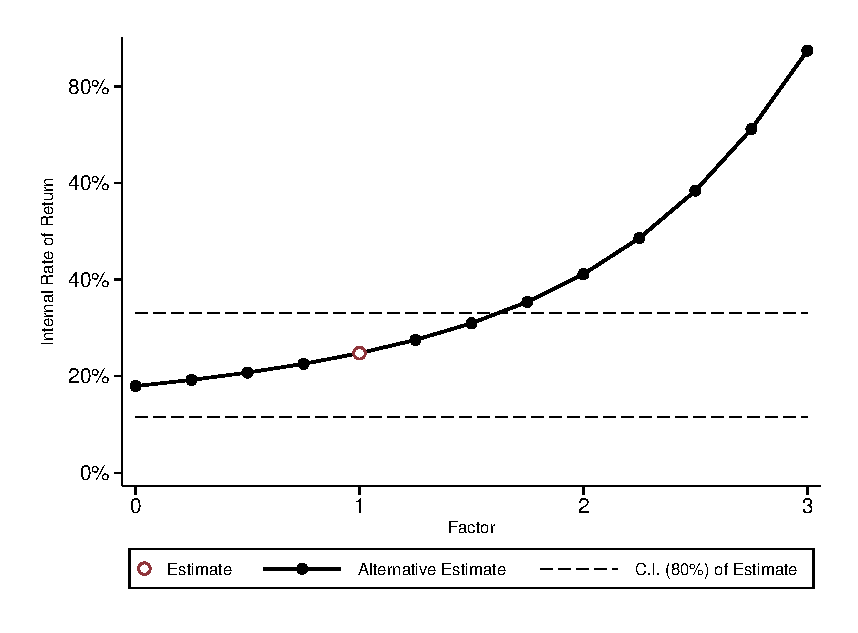
\includegraphics[width=\textwidth]{AppOutput/Sensitivity/irrf_cc_m1.eps}
	\end{subfigure}
	
	\floatfoot{
	\noindent Note: These graphs display how the internal rate of return changes
	for males as we multiply each component by a factor from 0 to 3. 
	The hollow circle represents our actual estimates, whereas the
	solid dots represent the alternative estimates we obtain by varying the 
	magnitude of each component. The estimates 
	presented in the paper are equal to the IRRs presented above when the multiplicative
	factor is equal to 1. The estimates are means of the empirical bootstrap 
	distribution. The 80\% confidence intervals are obtained by taking the 10\textsuperscript{th}
	and 90\textsuperscript{th} quantiles of the bootstrap distribution.
	}
\end{figure}

\noindent Figure \ref{fig:bcrf_factor_f} shows how the benefit/cost ratio changes for females as
we multiply each component of the benefits and costs by a factor between 0 and 3. We 
observe that the ratio is generally insensitive to changes in all the components, 
except parental income, labor income, education costs, and program costs. The sensitivity
to program costs is due to the fact that it is the denominator of the 
benefit/cost ratio. In the case of the other three components, when discounted, 
they exhibit the three largest present values. The sensitivity of the benefit/cost
ratio to changes in these components therefore indicates the magnitude of those 
components relative to the rest, with parental income having the largest magnitude
in terms of discounted treatment effect, followed by labor income, and then
education costs. 

\begin{figure}[H]
\caption{Benefit/cost Ratio vs.~Components, Females} \label{fig:bcrf_factor_f}

	\begin{subfigure}[h]{0.8\textwidth}
	\centering
	\caption{Labor Income} \label{fig:bcrf_inc_labor_f1}
	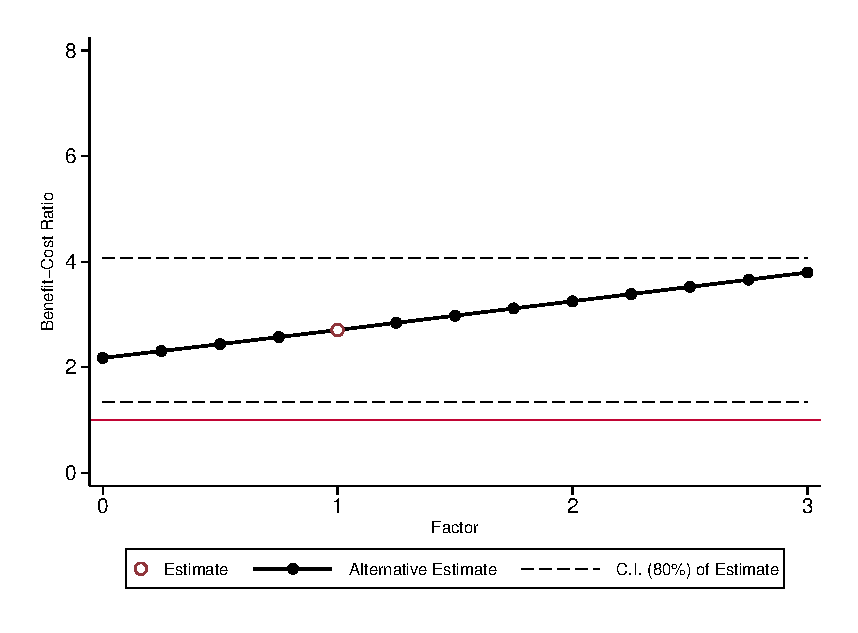
\includegraphics[width=\textwidth]{AppOutput/Sensitivity/bcrf_inc_labor_f1.eps}
	\end{subfigure}	
	
	\begin{subfigure}[h]{0.8\textwidth}
	\centering
	\caption{Public-Transfer Income} \label{fig:bcrf_transfer_f1}
	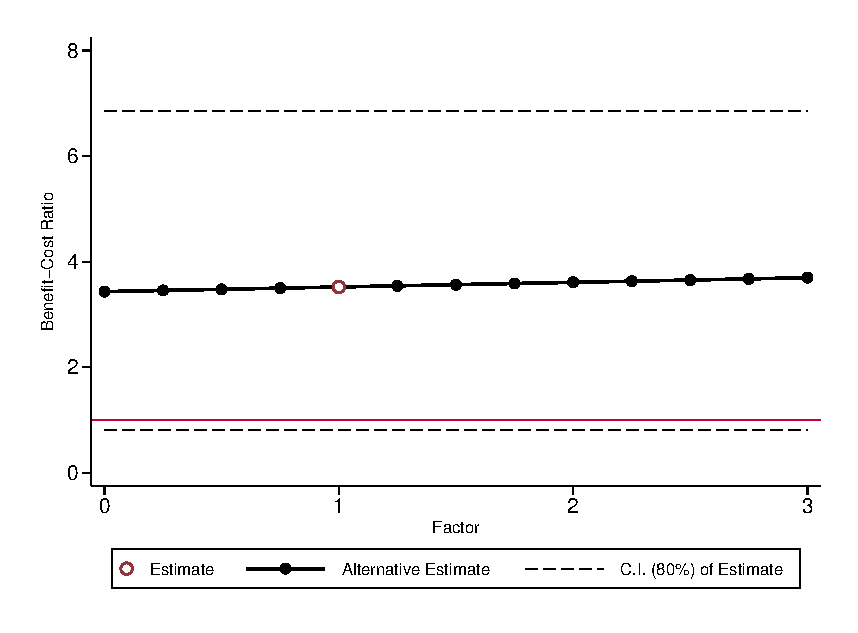
\includegraphics[width=\textwidth]{AppOutput/Sensitivity/bcrf_transfer_f1.eps}
	\end{subfigure}
\end{figure}
	
\begin{figure}[H]
\ContinuedFloat		
	\begin{subfigure}[h]{0.8\textwidth}
	\centering
	\caption{Parental Income} \label{fig:bcrf_inc_parent_f1}
	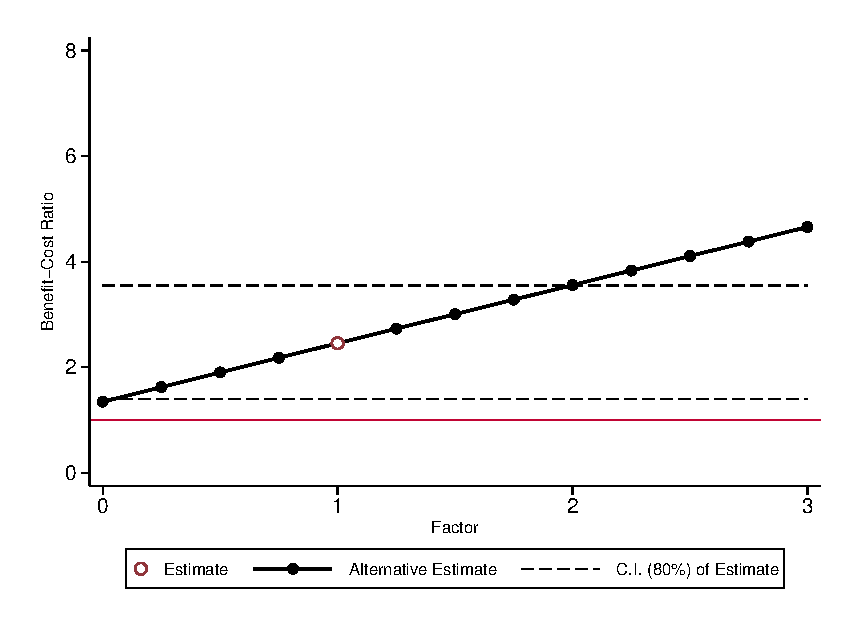
\includegraphics[width=\textwidth]{AppOutput/Sensitivity/bcrf_inc_parent_f1.eps}
	\end{subfigure}
	
	\begin{subfigure}[h]{0.8\textwidth}
	\centering
	\caption{Quality-Adjusted Life Years} \label{fig:bcrf_qaly_f1}
	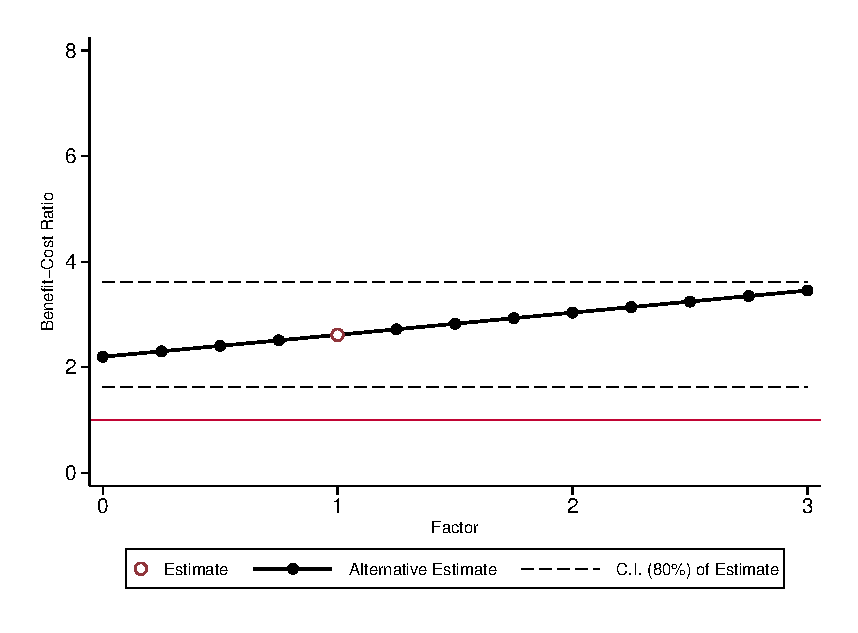
\includegraphics[width=\textwidth]{AppOutput/Sensitivity/bcrf_qaly_f1.eps}
	\end{subfigure}
\end{figure}
	
\begin{figure}[H]
\ContinuedFloat		
	\begin{subfigure}[h]{0.8\textwidth}
	\centering
	\caption{Health Costs} \label{fig:bcrf_health_f1}
	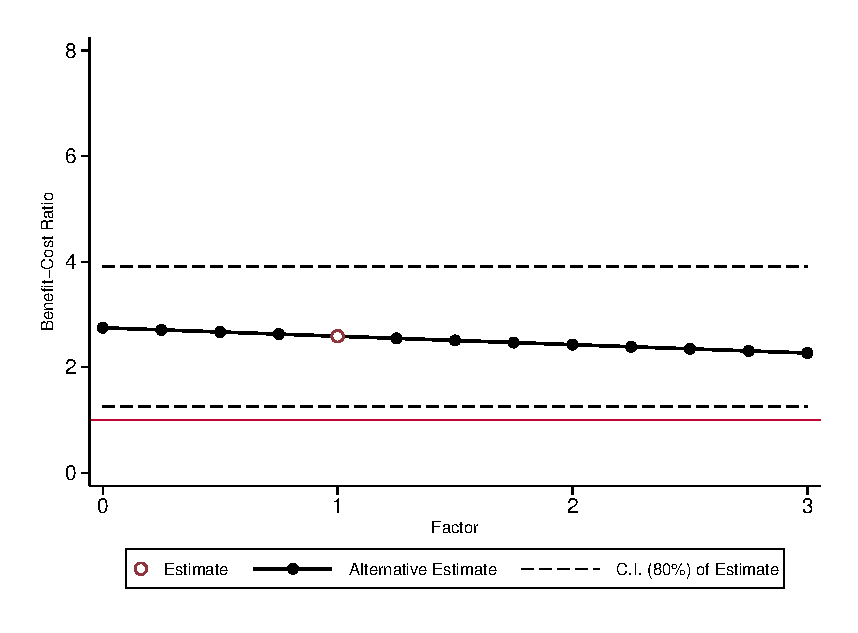
\includegraphics[width=\textwidth]{AppOutput/Sensitivity/bcrf_health_f1.eps}
	\end{subfigure}
	
	\begin{subfigure}[h]{0.8\textwidth}
	\centering
	\caption{Education Costs} \label{fig:bcrf_edu_f1}
	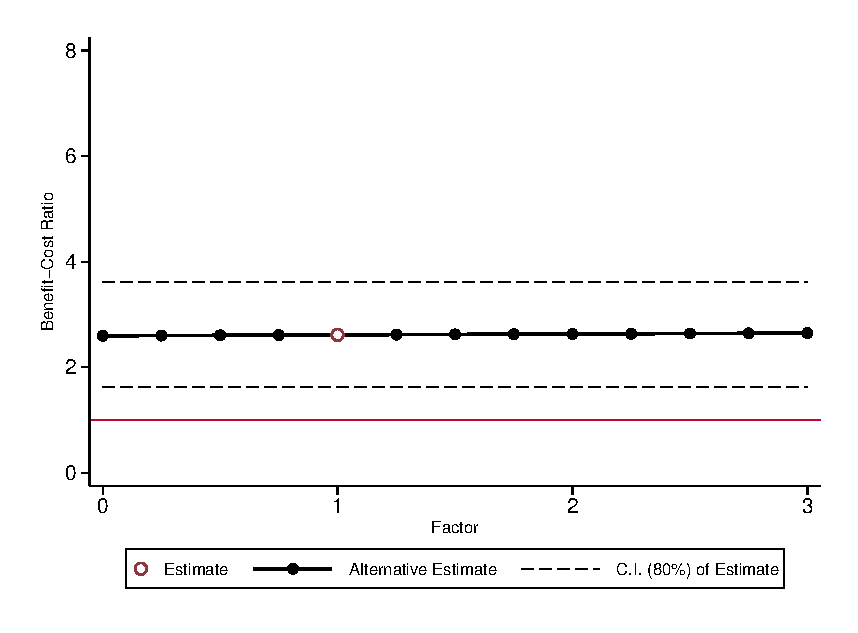
\includegraphics[width=\textwidth]{AppOutput/Sensitivity/bcrf_edu_f1.eps}
	\end{subfigure}
\end{figure}

\begin{figure}[H]
\ContinuedFloat			
	\begin{subfigure}[h]{0.8\textwidth}
	\centering
	\caption{Crime Costs} \label{fig:bcrf_crime_f1}
	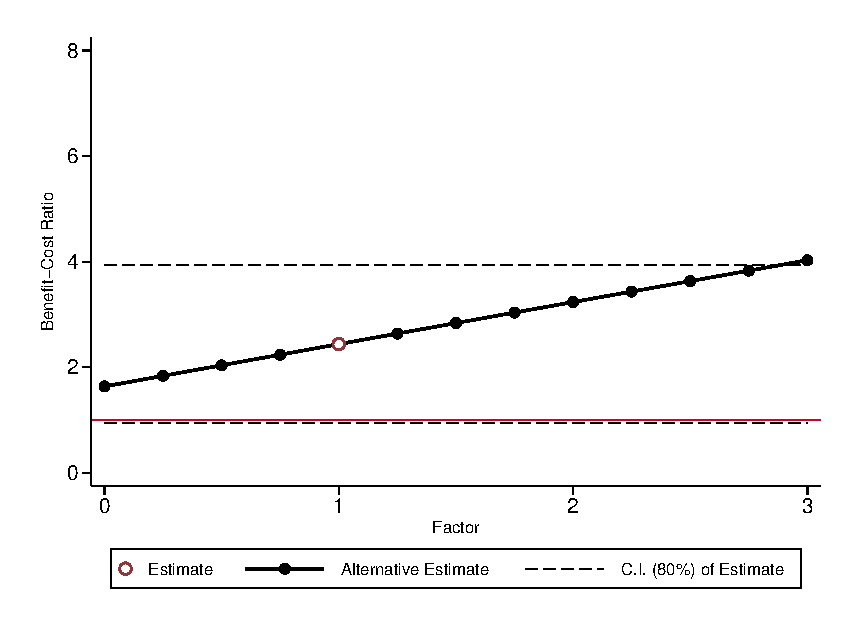
\includegraphics[width=\textwidth]{AppOutput/Sensitivity/bcrf_crime_f1.eps}
	\end{subfigure}
	
	\begin{subfigure}[h]{0.8\textwidth}
	\centering
	\caption{Program Costs} \label{fig:bcrf_costs_f1}
	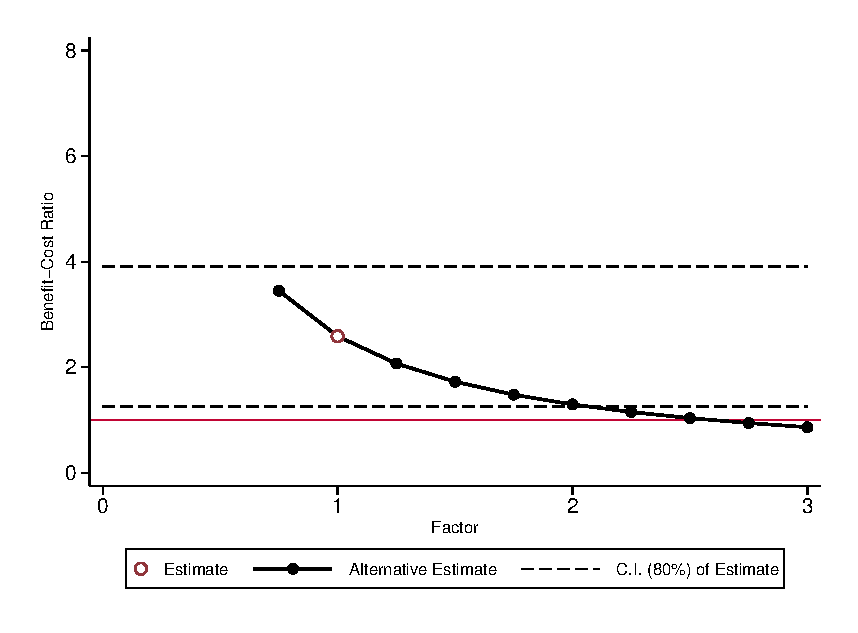
\includegraphics[width=\textwidth]{AppOutput/Sensitivity/bcrf_costs_f1.eps}
	\end{subfigure}
\end{figure}
	
\begin{figure}[H]
\ContinuedFloat		
	\begin{subfigure}[h]{0.8\textwidth}
	\centering
	\caption{Control Substitution Costs} \label{fig:bcrf_cc_f1}
	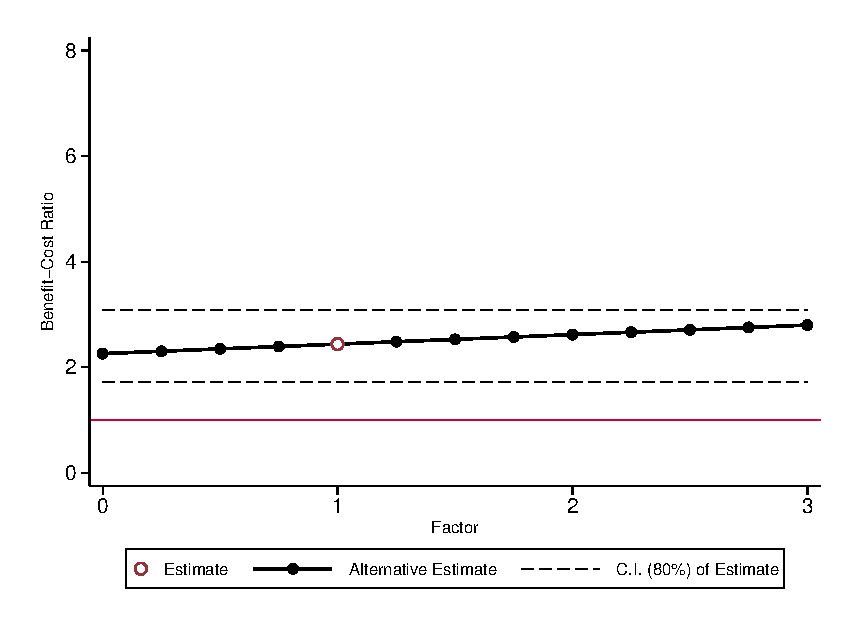
\includegraphics[width=\textwidth]{AppOutput/Sensitivity/bcrf_cc_f1.eps}
	\end{subfigure}
	
	\floatfoot{
	\noindent Note: These graphs display how the benefit/cost ratio changes
	for females as we multiply each component by a factor from 0 to 3. 
	The red line indicates a benefit/cost ratio of 1. 
	The hollow circle represents our actual estimates, whereas the
	solid dots represent the alternative estimates we obtain by varying the 
	magnitude of each component. The benefit/cost ratio 
	presented in the paper is equal to those presented above when the multiplicative
	factor is equal to 1. The estimates are means of the empirical bootstrap 
	distribution. The 80\% confidence intervals are obtained by taking the 10\textsuperscript{th}
	and 90\textsuperscript{th} quantiles of the bootstrap distribution.
	}
\end{figure}

\noindent Figure \ref{fig:bcrf_factor_m} displays how the benefit/cost ratio for males varies
as we multiply each component of the benefits and costs by a factor between 0 and 3.
We observe that the ratio is insensitive to the scaling of public-transfer income, health costs,
education costs, and control substitution costs. Barring program costs, the components that
vary the benefit/cost ratio the most are crime costs, parental income, labor income,
health expenditure, and QALYs, in that order. This is simply a result of the relevant 
magnitude of each of those components in the benefits stream after discounting. 


\begin{figure}[H]
\caption{Benefit/cost Ratio vs.~Components, Males} \label{fig:bcrf_factor_m}
	
	\begin{subfigure}[h]{0.8\textwidth}
	\centering
	\caption{Labor Income} \label{fig:bcrf_inc_labor_m1}
	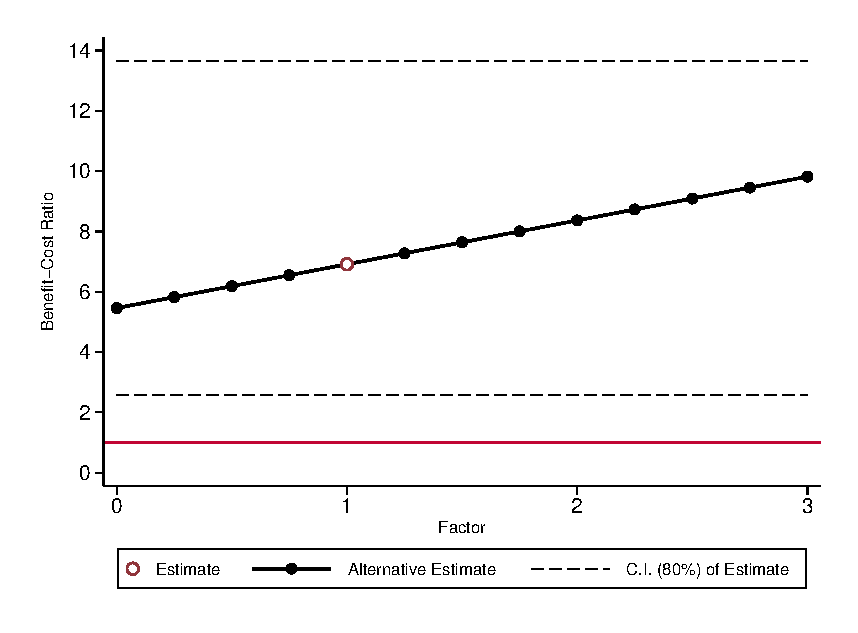
\includegraphics[width=\textwidth]{AppOutput/Sensitivity/bcrf_inc_labor_m1.eps}
	\end{subfigure}
	
	\begin{subfigure}[h]{0.8\textwidth}
	\centering
	\caption{Public-Transfer Income} \label{fig:bcrf_transfer_m1}
	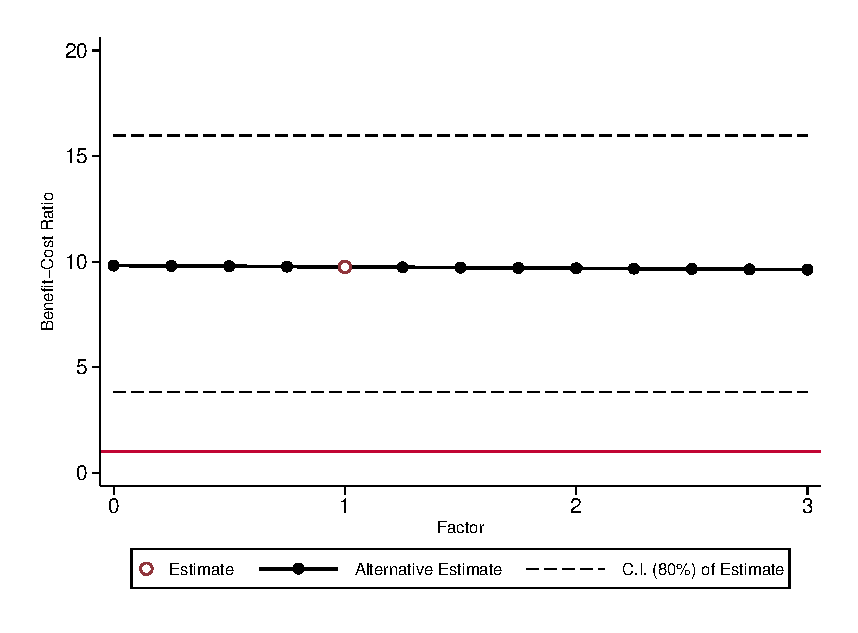
\includegraphics[width=\textwidth]{AppOutput/Sensitivity/bcrf_transfer_m1.eps}
	\end{subfigure}
\end{figure}

\begin{figure}[H]
\ContinuedFloat		
	\begin{subfigure}[h]{0.8\textwidth}
	\centering
	\caption{Parental Income} \label{fig:bcrf_inc_parent_m1}
	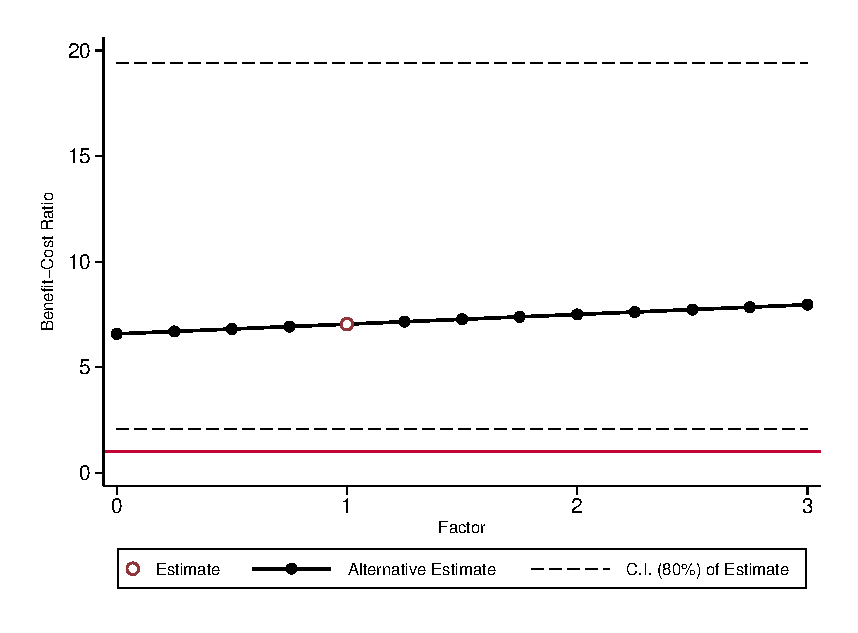
\includegraphics[width=\textwidth]{AppOutput/Sensitivity/bcrf_inc_parent_m1.eps}
	\end{subfigure}
	
	\begin{subfigure}[h]{0.8\textwidth}
	\centering
	\caption{Quality-Adjusted Life Years} \label{fig:bcrf_qaly_m1}
	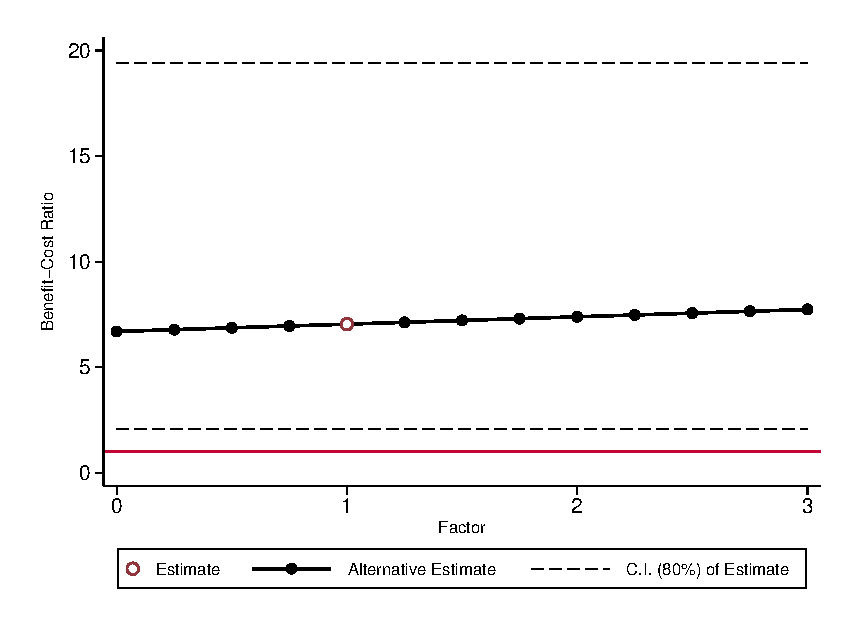
\includegraphics[width=\textwidth]{AppOutput/Sensitivity/bcrf_qaly_m1.eps}
	\end{subfigure}
\end{figure}


\begin{figure}[H]
\ContinuedFloat	
	\begin{subfigure}[h]{0.8\textwidth}
	\centering
	\caption{Health Costs} \label{fig:bcrf_health_m1}
	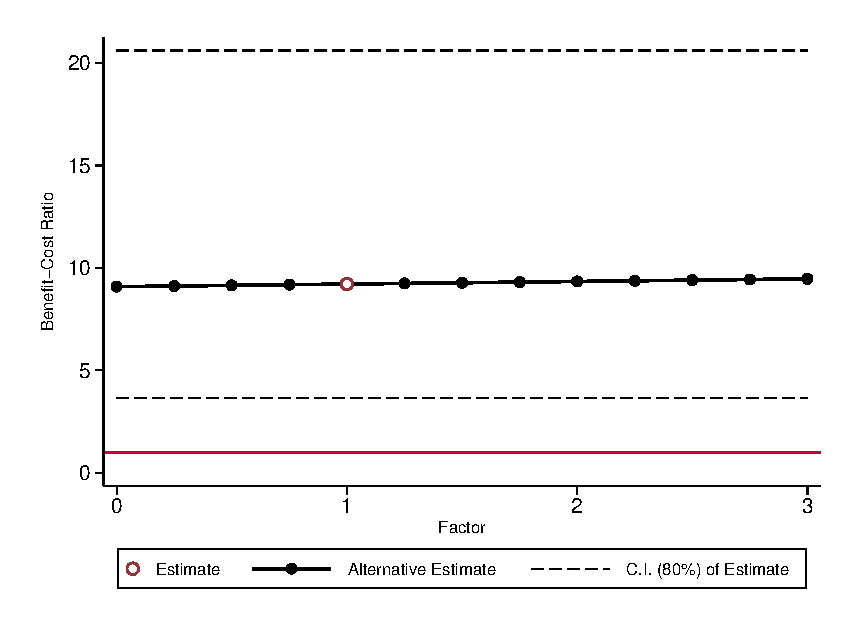
\includegraphics[width=\textwidth]{AppOutput/Sensitivity/bcrf_health_m1.eps}
	\end{subfigure}
	
	\begin{subfigure}[h]{0.8\textwidth}
	\centering
	\caption{Education Costs} \label{fig:bcrf_edu_m1}
	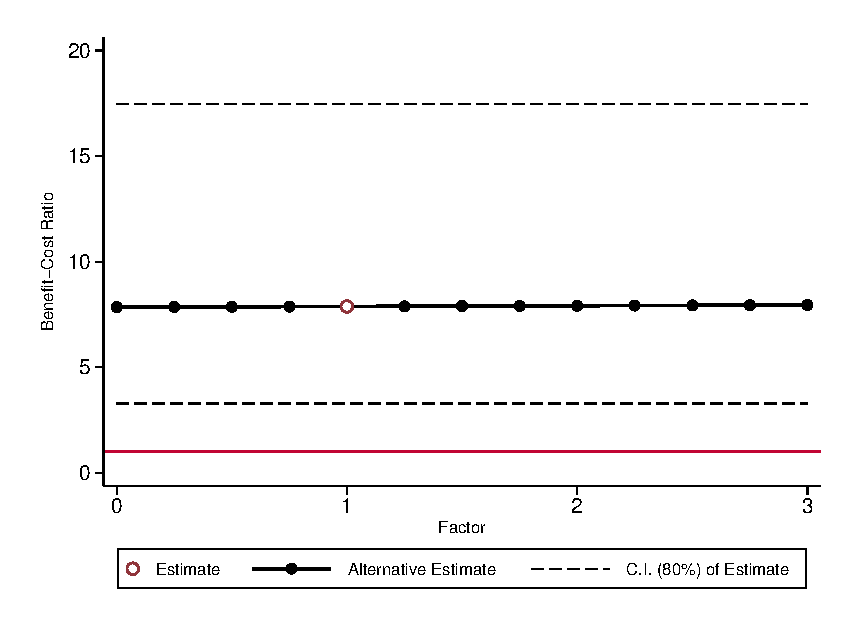
\includegraphics[width=\textwidth]{AppOutput/Sensitivity/bcrf_edu_m1.eps}
	\end{subfigure}
\end{figure}	


\begin{figure}[H]
\ContinuedFloat		
	\begin{subfigure}[h]{0.8\textwidth}
	\centering
	\caption{Crime Costs} \label{fig:bcrf_crime_m1}
	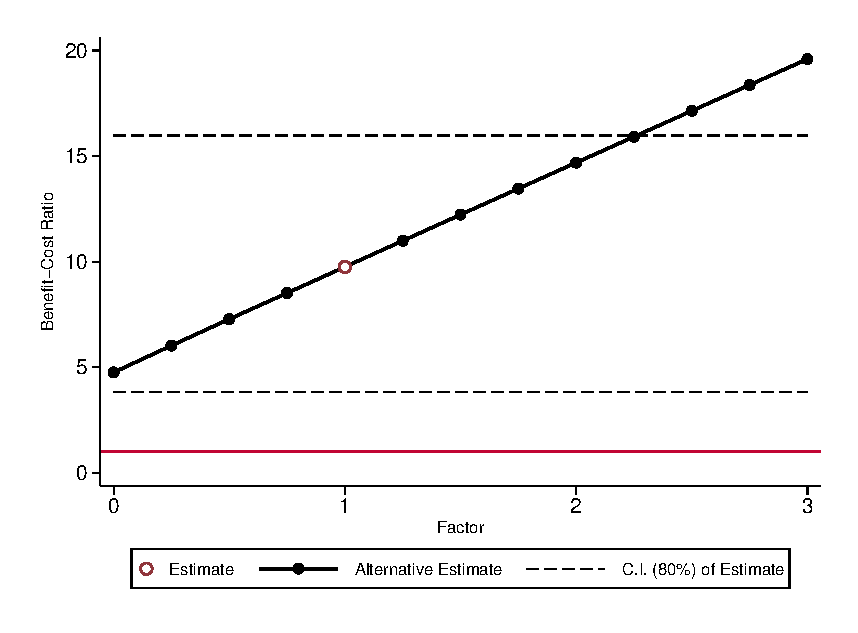
\includegraphics[width=\textwidth]{AppOutput/Sensitivity/bcrf_crime_m1.eps}
	\end{subfigure}
	
	\begin{subfigure}[h]{0.8\textwidth}
	\centering
	\caption{Program Costs} \label{fig:bcrf_costs_m1}
	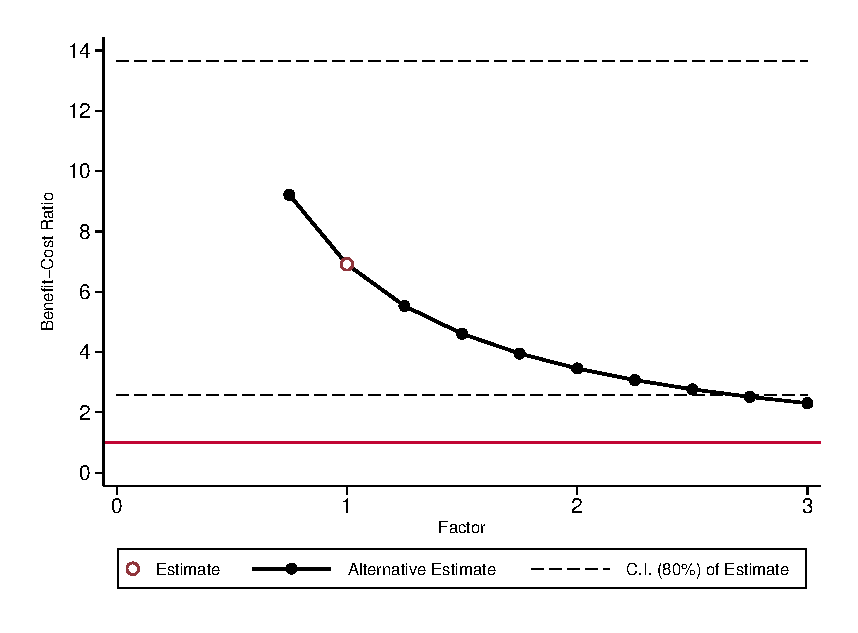
\includegraphics[width=\textwidth]{AppOutput/Sensitivity/bcrf_costs_m1.eps}
	\end{subfigure}
\end{figure}

	
\begin{figure}[H]
\ContinuedFloat		
	\begin{subfigure}[h]{0.8\textwidth}
	\centering
	\caption{Control Substitution Costs} \label{fig:bcrf_cc_m1}
	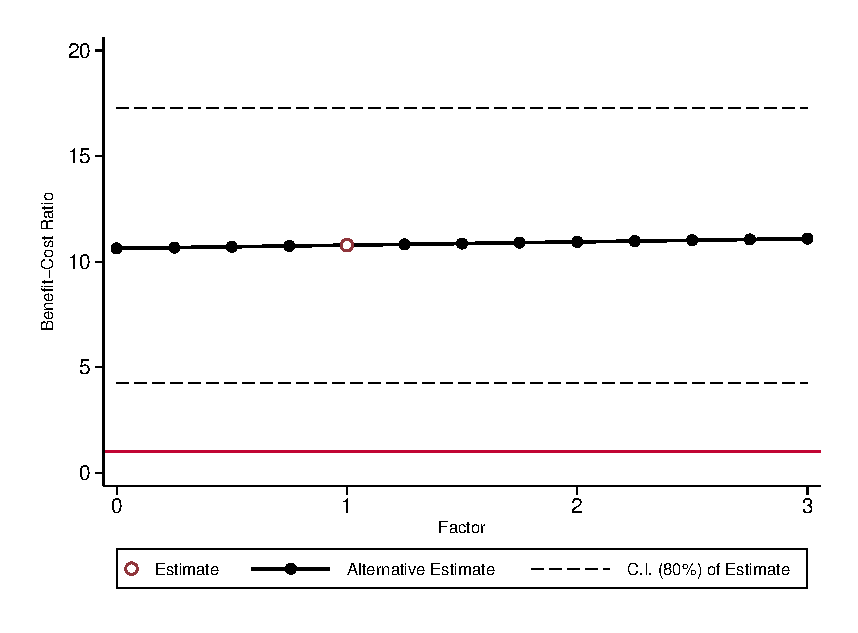
\includegraphics[width=\textwidth]{AppOutput/Sensitivity/bcrf_cc_m1.eps}
	\end{subfigure}
	
	\floatfoot{
	\noindent Note: These graphs display how the benefit/cost ratio changes
	for males as we multiply each component by a factor from 0 to 3. 
	The red line indicates a benefit/cost ratio of 1. 
	The hollow circle represents our actual estimates, whereas the
	solid dots represent the alternative estimates we obtain by varying the 
	magnitude of each component. The benefit/cost ratio 
	presented in the paper is equal to those presented above when the multiplicative
	factor is equal to 1. The estimates are means of the empirical bootstrap 
	distribution. The 80\% confidence intervals are obtained by taking the 10\textsuperscript{th}
	and 90\textsuperscript{th} quantiles of the bootstrap distribution.
	}
\end{figure}

\noindent Overall, we find the benefit/cost ratio to be stable across changes in the data, 
as well as changes in our assumptions regarding the discount rate and the marginal
cost of welfare. The IRR tends to be more sensitive to changes in the data
and assumptions.
